In the posterior predictive model checking of this study (Section~\ref{subsec:wo Layers of Model Checking}), we found that the \textbf{maximum survey duration $A$}, controlling the censoring mechanism in Algorithm 1 through the reparameterization $A$, has a substantial influence on simulation outcomes and the credibility of posterior predictive results. $A$ sets the observation window in simulation, thereby determining both the censoring rate and the distribution of event times.

This quantity is not estimated by the model but specified externally when generating fake data. Although it may appear auxiliary, it is tightly coupled with model checking: different choices of $A$ change the censoring structure in simulated data and can alter conclusions from posterior predictive checks.

Does the observed data carry information about $A$? Yes. In any survival dataset, the “shadow” of the survey window is reflected in the censoring proportion and the shape of the observed durations. If $A$ is small, many subjects are censored before the event occurs, leading to a high right-censoring rate and “compressed” event times. Conversely, a large $A$ yields more observed events, lower censoring, and more dispersed event times.

This can be seen in Figure~\ref{fig:离职数据分开的直方图}, which separates event and censored durations in the employee turnover data. The number of events and censors is roughly balanced, suggesting that the survey was long enough to capture about half of the departures. Since the maximum observed duration exceeds 170 months, it is reasonable to infer that the underlying survey duration $A$ should be at least greater than 170 months. While this observation alone does not pinpoint $A$, exploratory simulations suggest that a value in the vicinity of 200 months yields censoring patterns most consistent with the observed data. This directly informs how the censoring mechanism should be set in simulation, and shows that implausibly small (e.g., $A=30$) or unrealistically large (e.g., $A=1000$) values can lead to misleading posterior predictive fits. In a Bayesian framework, such information about $A$ will naturally be reflected in its posterior distribution when $A$ is included in the likelihood, which is the focus of the next section.
\begin{figure}[H]
    \centering
    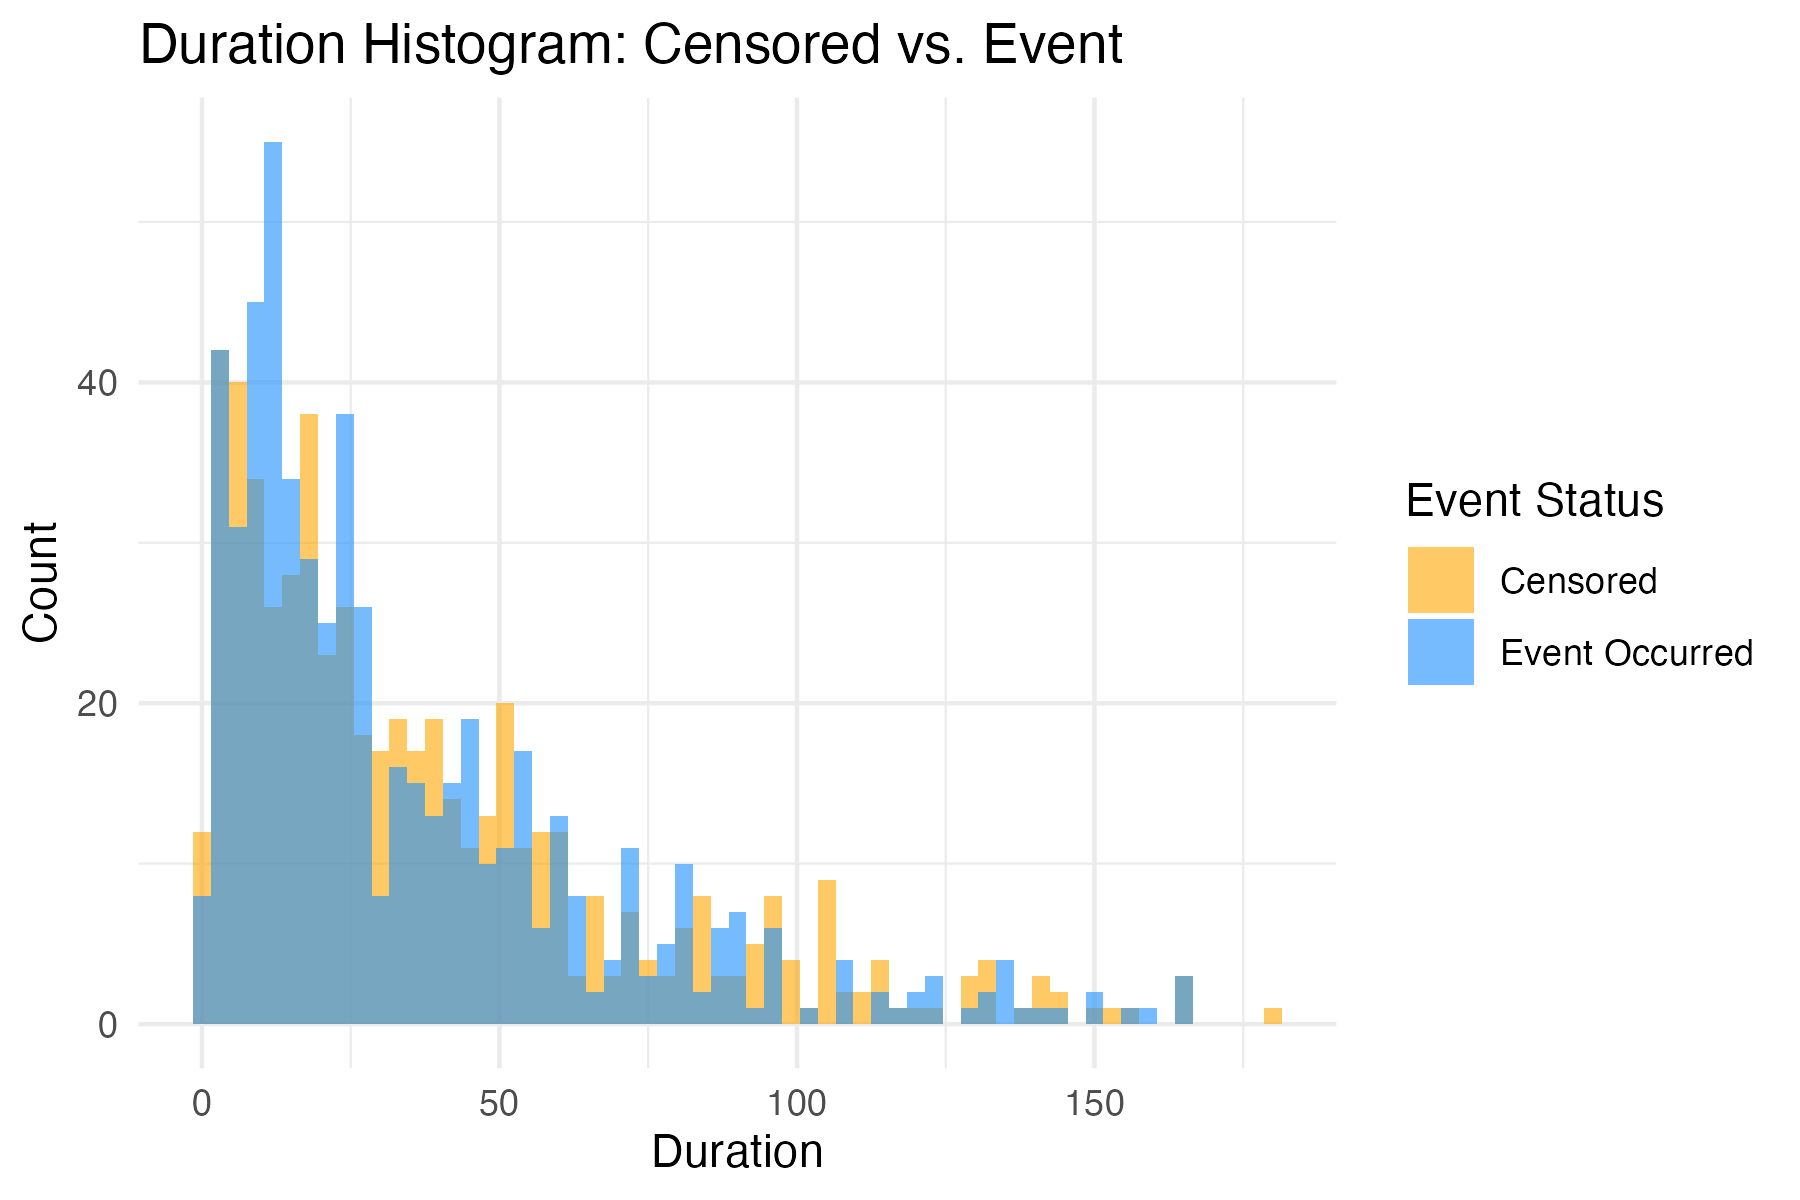
\includegraphics[height=5.5cm, width=0.6\textwidth]{images/separate_hist.png}
    \caption{Histograms of censored and event durations in the employee turnover data}
    \label{fig:离职数据分开的直方图}
\end{figure}
To illustrate the effect of unrealistic observation windows, we simulate under two settings, $A = 30$ and $A = 1000$, and plot the empirical cumulative distribution functions (ECDFs) for both the event subsample ($\delta = 1$) and the censored subsample ($\delta = 0$), along with the histograms of simulated durations.
\begin{itemize}
    \item $A = 30$ (Figure~\ref{fig:ppc-A30}). Compared to the real-data histogram (Figure~\ref{fig:离职数据分开的直方图}), the simulated durations in Figure~\ref{fig:fake-hist_a30} are heavily compressed within 0–30 months, indicating that both events and censorings occur unusually early. Correspondingly, the ECDFs for events and censorings (Figure~\ref{fig:ecdf-cens_a30}~\ref{fig:ecdf-event_a30}, red lines) rise too steeply at short durations, deviating noticeably from the observed curves. This mismatch is primarily driven by an unrealistic observation window $A$, rather than a misfit of the event-time distribution (e.g., the parameter $\lambda$) itself. This mismatch is driven by an unrealistic $A$, rather than by misestimation of the event-time parameter $\lambda$
    \item $A = 1000$ (Figure~\ref{fig:ppc-A1000})
  In contrast, Figure~\ref{fig:fake-hist_a1000} shows a histogram with a much wider and sparser spread of durations, and the ECDF curves (Figure~\ref{fig:ecdf-event_a1000}~\ref{fig:ecdf-cens_a1000}, red lines) align more closely with the observed data. However, when compared to the real-data histogram in Figure~\ref{fig:离职数据分开的直方图}, this setting exceeds any realistic survey length, implying a maximum tenure close to 83 years, which is implausible in practical employment contexts. Thus, although the simulated curves fit better visually, this apparent “match” relies on an unrealistic assumption about $A$, and should not be accepted as a reliable model-checking result.
\end{itemize}
These examples reinforce a key point: posterior predictive fit must be judged alongside the plausibility of the data-generating assumptions. Identifying a realistic range for $A$ is not only essential for credible model checking but also motivates the next step of our study—explicitly incorporating $A$ into the likelihood to estimate it jointly with the event-time parameters.
\begin{figure}[htbp]
\centering
\begin{subfigure}[t]{0.32\textwidth}
  \centering
  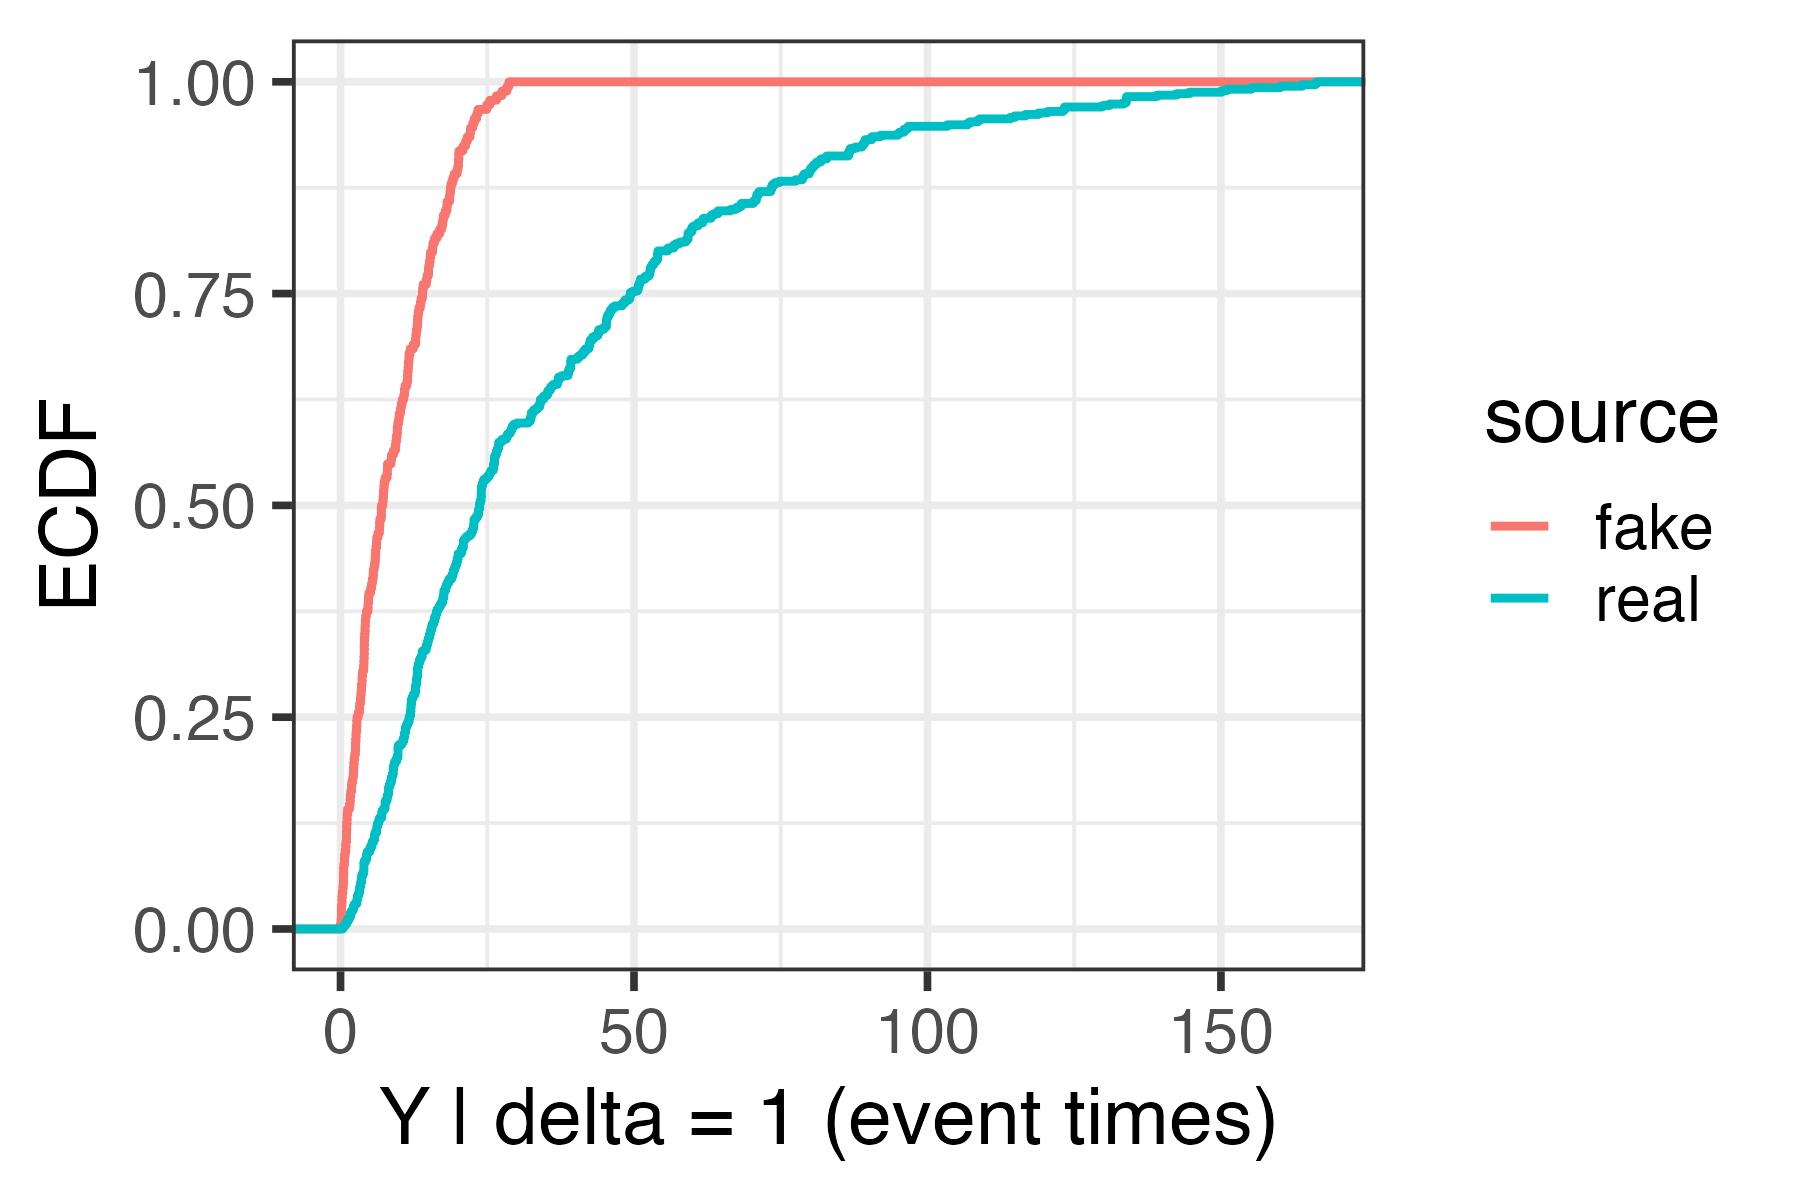
\includegraphics[width=\linewidth]{images/ppc_event_ecdf_A30.png}  % 图1路径
  \caption{ECDF of $Y \mid \delta=1$}
  \label{fig:ecdf-event_a30}
\end{subfigure}\hfill
\begin{subfigure}[t]{0.32\textwidth}
  \centering
  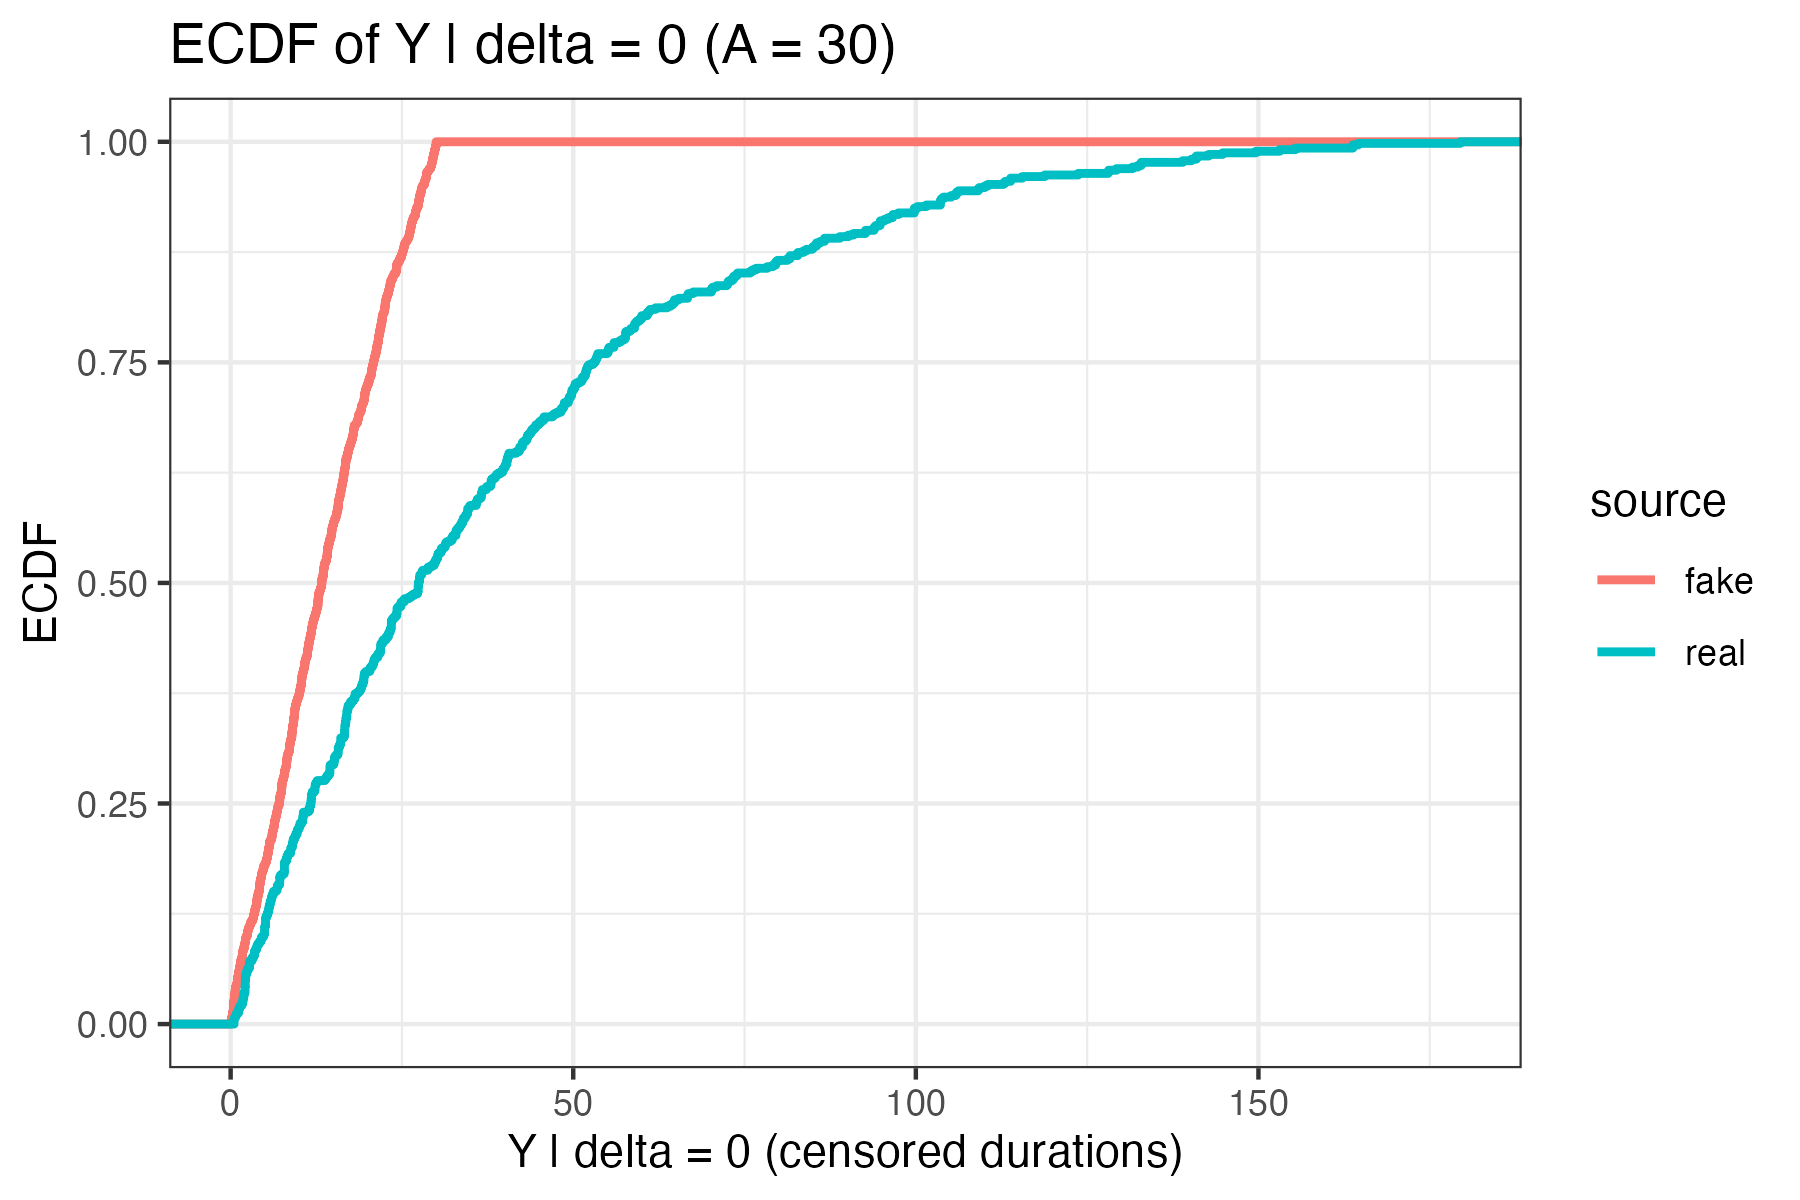
\includegraphics[width=\linewidth]{images/ppc_censored_ecdf_A30.png}   
  \caption{ECDF of $Y \mid \delta=0$}
  \label{fig:ecdf-cens_a30}
\end{subfigure}\hfill
\begin{subfigure}[t]{0.35\textwidth}
  \centering
  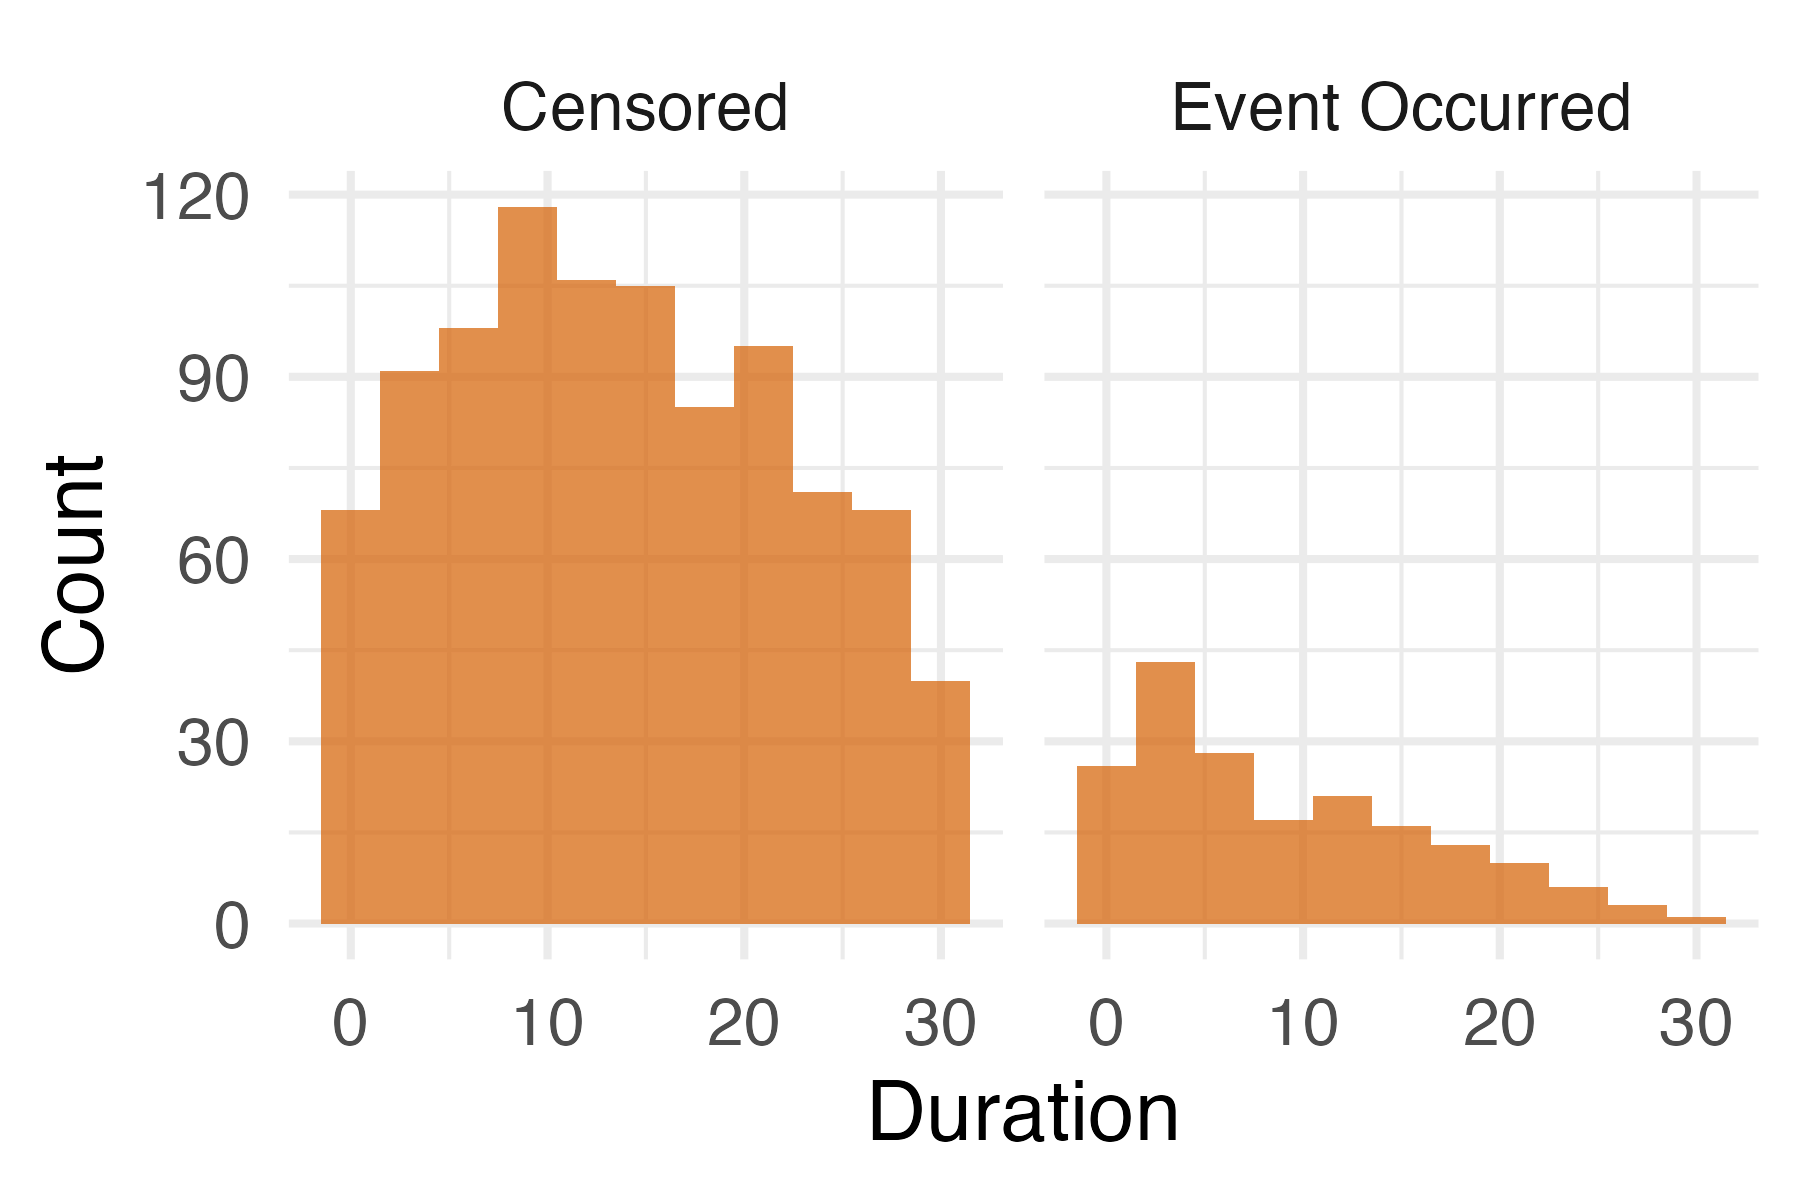
\includegraphics[width=\linewidth]{images/fake_duration_hist_a30.png}   % 图3路径
  \caption{Fake-data histogram}
  \label{fig:fake-hist_a30}
\end{subfigure}
\caption{Posterior predictive checking ($A=30$).}
\label{fig:ppc-A30}
\end{figure}
%%%%%%%%%%%%%%%%%%%%%%
\begin{figure}[htbp]
\centering
\begin{subfigure}[t]{0.3\textwidth}
  \centering
  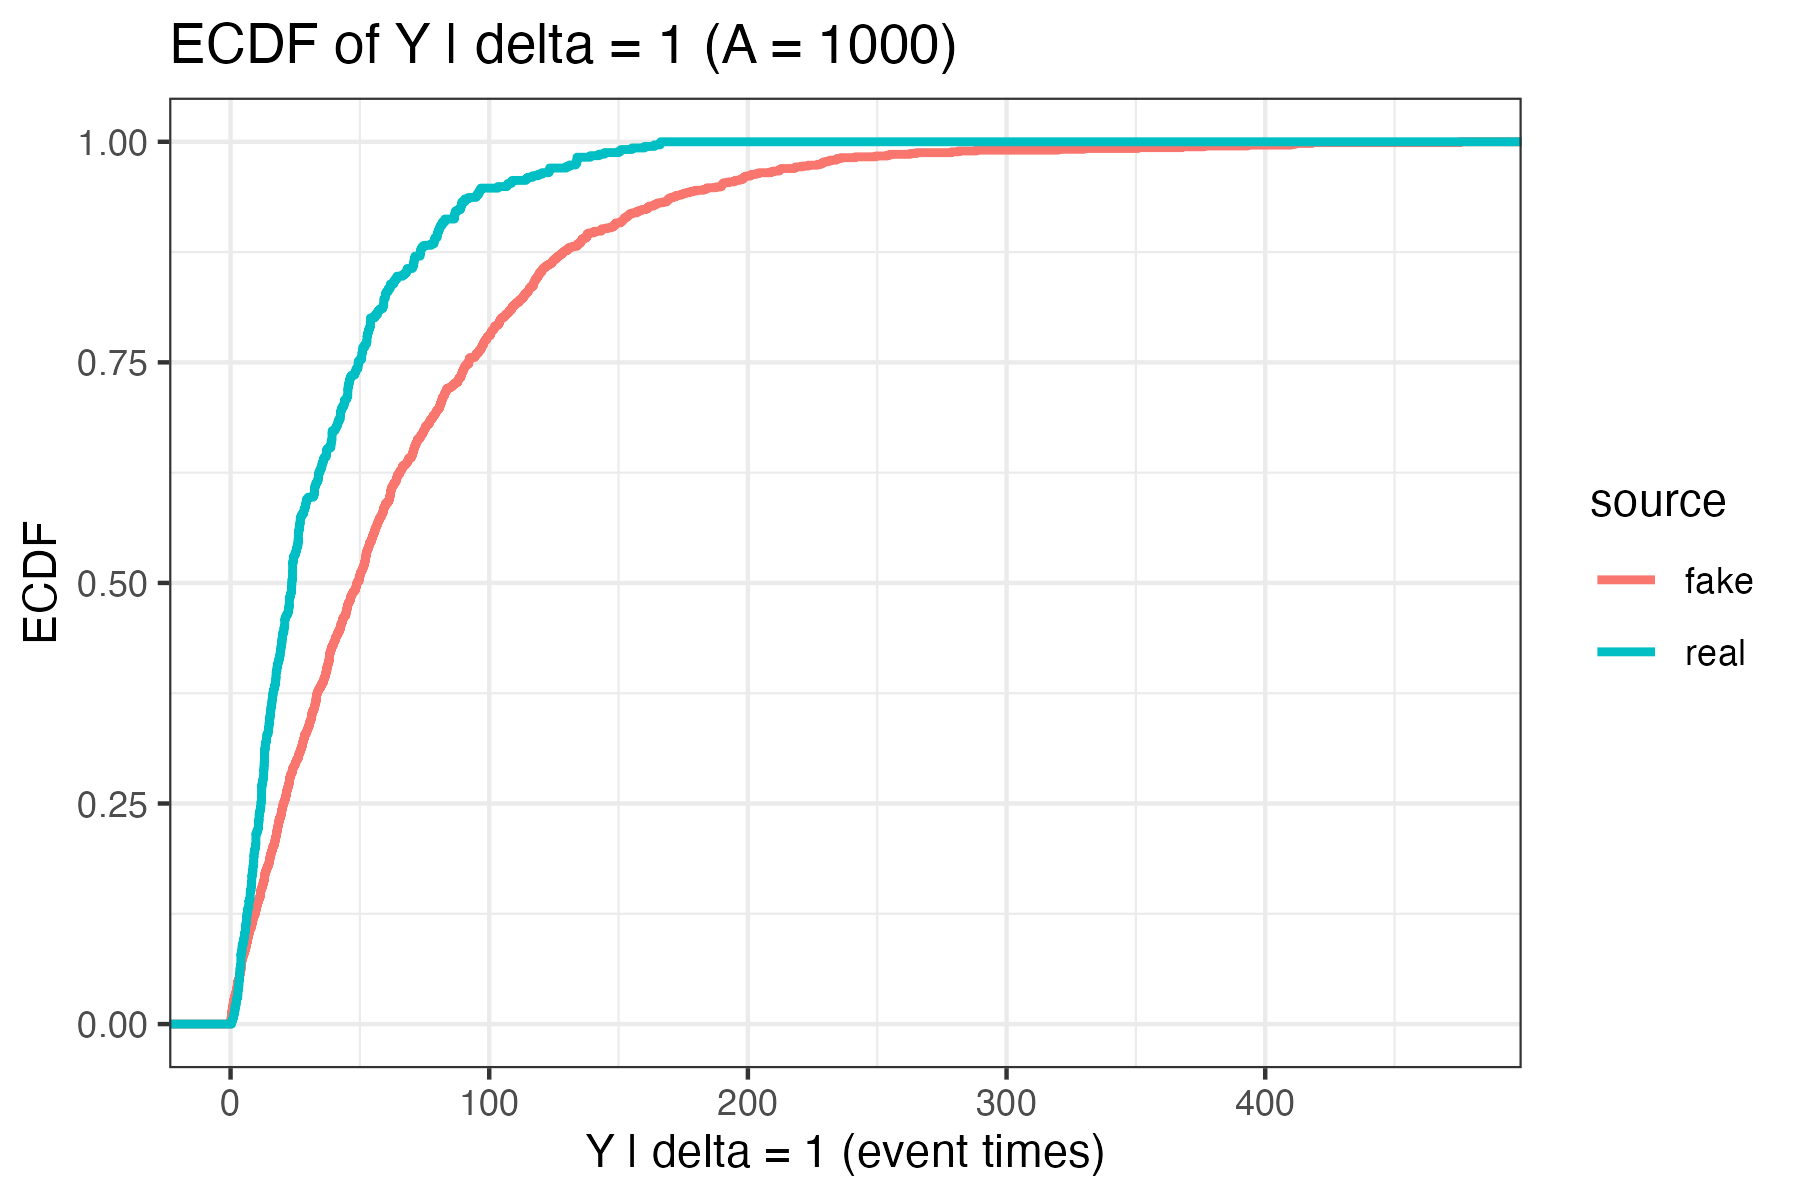
\includegraphics[width=\linewidth]{images/ppc_event_ecdf_A1000.png}  % 图1路径
  \caption{ECDF of $Y \mid \delta=1$}
  \label{fig:ecdf-event_a1000}
\end{subfigure}\hfill
\begin{subfigure}[t]{0.3\textwidth}
  \centering
  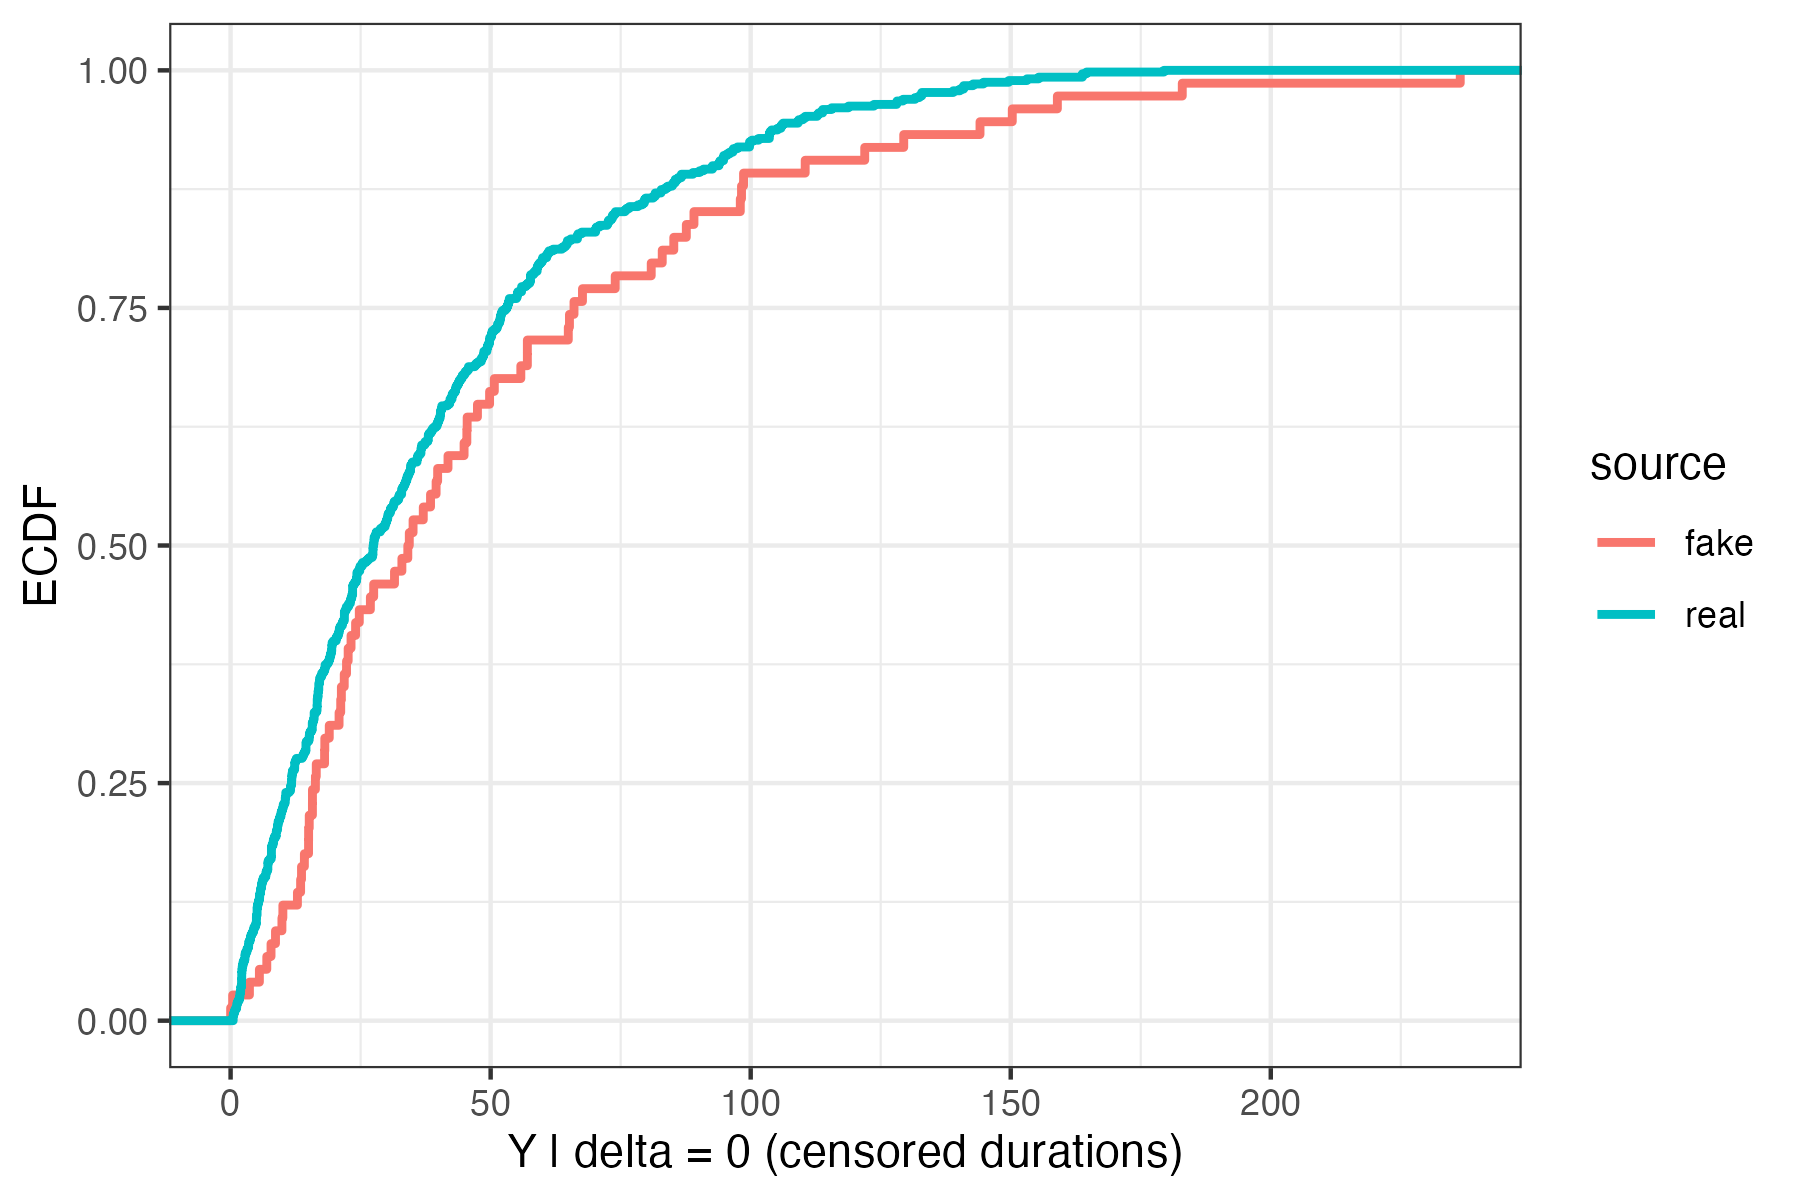
\includegraphics[width=\linewidth]{images/ppc_censored_ecdf_A1000.png} 
  \caption{ECDF of $Y \mid \delta=0$}
  \label{fig:ecdf-cens_a1000}
\end{subfigure}\hfill
\begin{subfigure}[t]{0.37\textwidth}
  \centering
  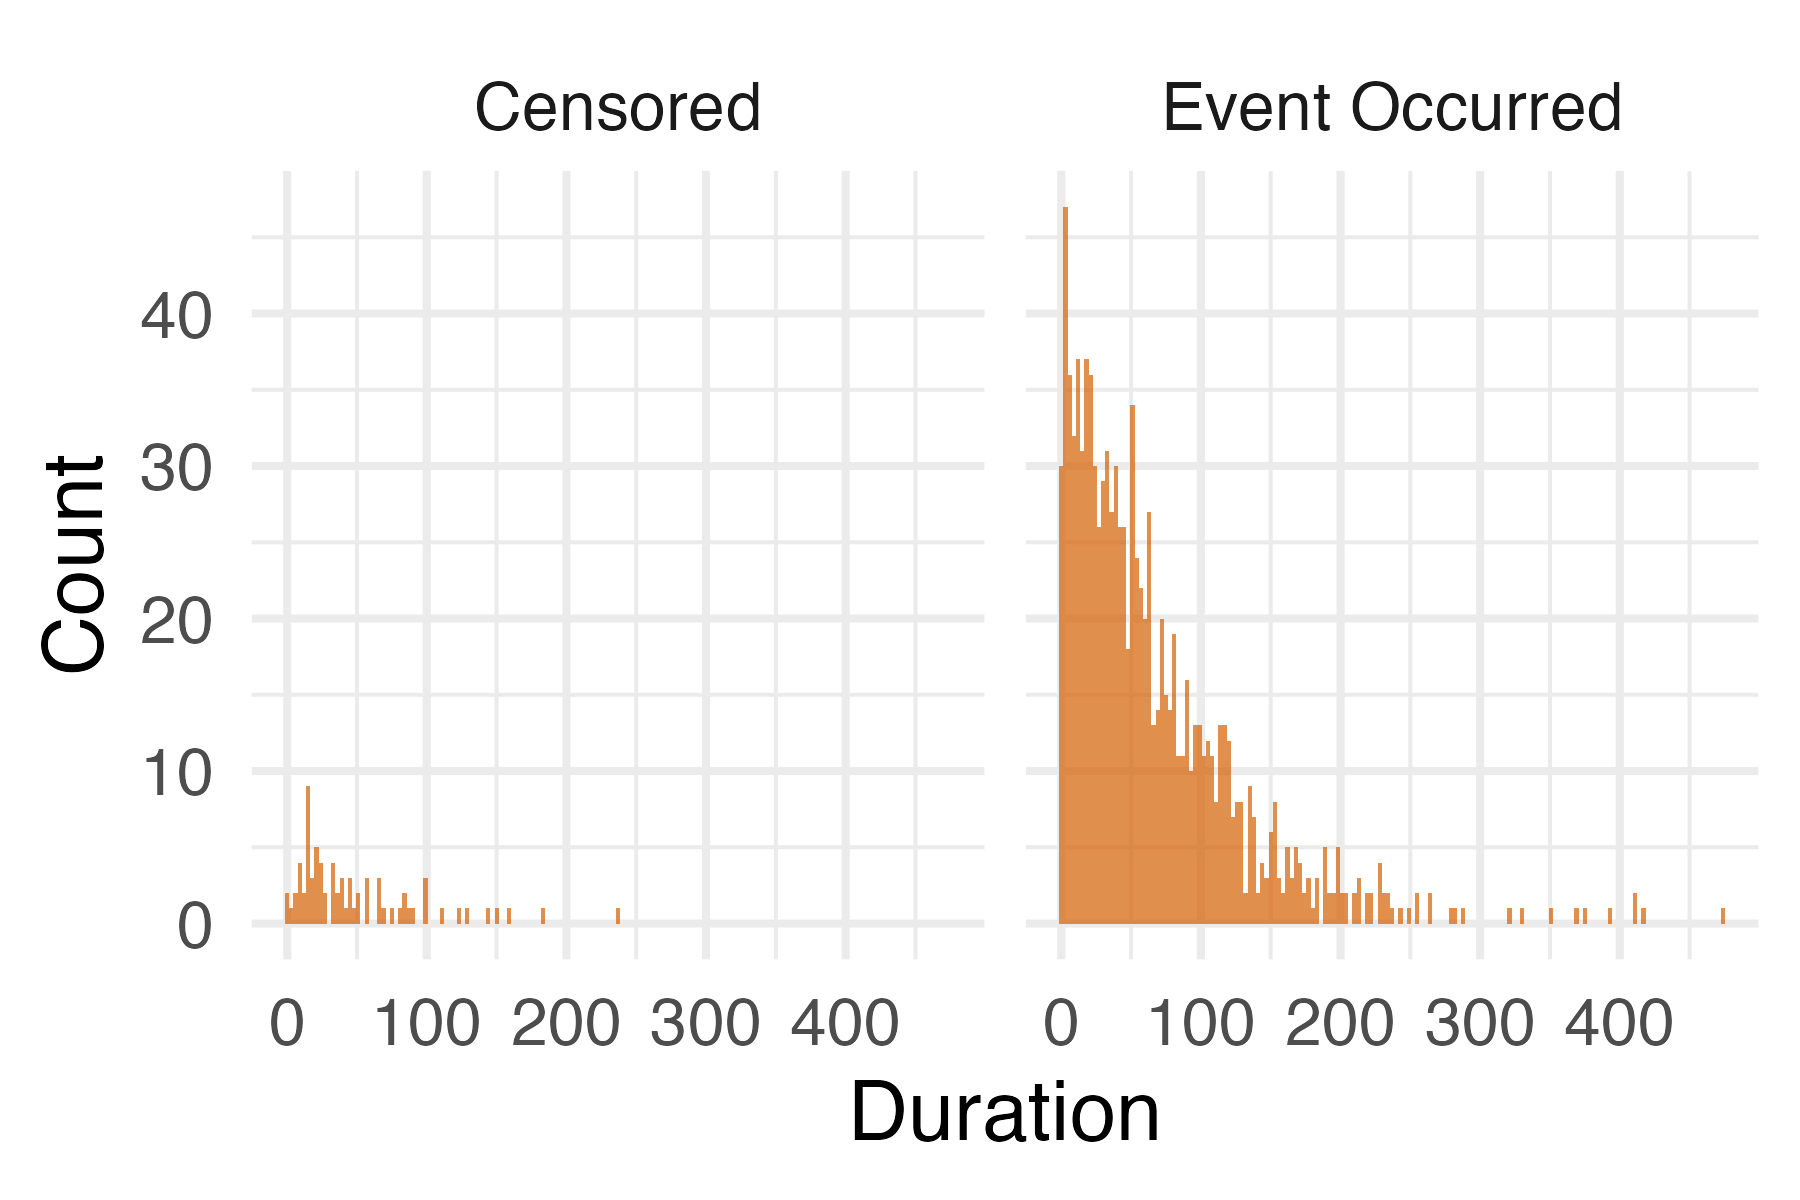
\includegraphics[width=\linewidth]{images/fake_duration_hist_a1000.png}   % 图3路径
  \caption{Fake-data histogram}
  \label{fig:fake-hist_a1000}
\end{subfigure}
\caption{Posterior predictive checking ($A=1000$).}
\label{fig:ppc-A1000}
\end{figure}
